\documentclass[a4paper, 11pt]{article}
\usepackage[slovene]{babel}
\usepackage[utf8]{inputenc}
\usepackage[T1]{fontenc}
\usepackage{lmodern}
\usepackage{amsmath, amssymb}
\usepackage{graphicx}
\usepackage{float}
\usepackage{caption}
\usepackage{subcaption}
\usepackage{hyperref}
\usepackage{listings}
\usepackage{xcolor}

\title{Vaja 2 -- Uporaba genetskega algoritma za optimizacijo izraza}
\author{Ime in priimek: \textbf{Gašper Leskovec} \\
Predmet: Inteligentni sistemi za podporo odločanju \\
Datum: \today}
\date{}

% Nastavitve za pravilen prikaz slovenskih šumnikov (č, š, ž) v prilogi s
% kodo: paket listings privzeto ne razume večbajtnih UTF-8 znakov, zato je
% poleg fontenc/lmodern potreben eksploziten "literate" nabor.
\lstset{
  basicstyle=\ttfamily\small,
  backgroundcolor=\color{black!5},
  frame=single,
  captionpos=b,
  numbers=left,
  numberstyle=\tiny,
  breaklines=true,
  tabsize=2,
  extendedchars=true,
  literate=%
    {č}{{\v{c}}}1 {š}{{\v{s}}}1 {ž}{{\v{z}}}1
    {Č}{{\v{C}}}1 {Š}{{\v{S}}}1 {Ž}{{\v{Z}}}1
    {á}{{\'a}}1 {é}{{\'e}}1 {í}{{\'i}}1 {ó}{{\'o}}1 {ú}{{\'u}}1
}

\begin{document}

\maketitle

\section{Uvod}
Cilj naloge je poiskati aritmetični izraz, sestavljen iz števk 1--9 in osnovnih operacij (+, --, *, /), katerega vrednost ustreza izbrani ciljni vrednosti. Iskanje je izvedeno z genetskim algoritmom (GA), brez uporabe vgrajenih Matlabovih orodij za optimizacijo.

\section{Opis naloge in metode}
Rešitev je predstavljena kot zaporedje izmenjujočih se števk in operatorjev (npr. \texttt{5+7+9+4*8}) dolžine, ki jo določa parameter \texttt{max\_terms}. Uporabnik ob zagonu poda ciljno vrednost in največje število členov izraza; velikost populacije, največje število generacij in verjetnost mutacije so nastavljene kot konstante na vrhu skripte.

Algoritem sledi standardni zgradbi genetskega algoritma:
\begin{itemize}
  \item \textbf{Inicializacija:} začetna populacija je sestavljena iz naključno generiranih izrazov ustrezne dolžine.
  \item \textbf{Ocenjevanje:} vsak izraz se ovrednoti (z varno obravnavo neveljavnih izrazov, npr. deljenja z 0); kriterijska funkcija je definirana kot $1/(1+|cilj - vrednost|)$, kar da vrednost 1 pri natančnem zadetku in gladko pada proti 0 z oddaljenostjo od cilja.
  \item \textbf{Selekcija:} starši za naslednjo generacijo se izbirajo z metodo ruletnega kolesa, kjer je verjetnost izbire osebka sorazmerna z njegovo kriterijsko funkcijo.
  \item \textbf{Križanje:} dva starša tvorita dva otroka z izmenjavo delov izraza na naključni točki.
  \item \textbf{Mutacija:} vsak gen (števka ali operator) se z verjetnostjo \texttt{mutation\_prob} naključno spremeni, kar vzdržuje diverziteto populacije.
  \item \textbf{Elitizem:} najboljši osebek generacije se nespremenjen prenese naprej, zato najboljša dosežena kriterijska funkcija nikoli ne pade.
\end{itemize}

Postopek se ponavlja do največjega dovoljenega števila generacij ali dokler algoritem ne najde izraza, ki natančno doseže ciljno vrednost.

\section{Rezultati glavnega zagona}
Glavni zagon je izveden s parametri: ciljna vrednost 53, \texttt{max\_terms} 5, populacija 20, \texttt{max\_generations} 100, \texttt{mutation\_prob} 0.1.

\begin{table}[H]
\centering
\begin{tabular}{|c|l|c|c|}\hline
Generacija & Izraz & Vrednost & Kriterijska funkcija \\ \hline
1 & 3*5*3+7/9 & 45.7778 & 0.1216 \\ \hline
2 & 3+5*9+7/9 & 48.7778 & 0.1915 \\ \hline
3 & 6+7+9+4*8 & 54.0000 & 0.5000 \\ \hline
4 & 6+7+9+4*8 & 54.0000 & 0.5000 \\ \hline
5 & 5+7+9+4*8 & 53.0000 & 1.0000 \\ \hline
\end{tabular}

\caption{Najboljša rešitev po generacijah (glavni zagon)}
\end{table}

\begin{figure}[H]
\centering
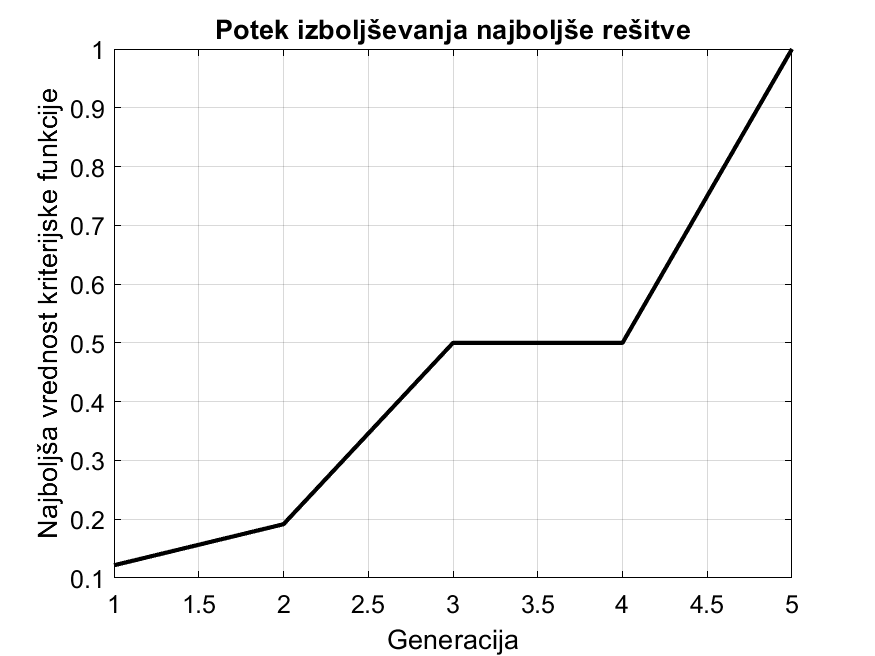
\includegraphics[width=0.8\textwidth]{figs/potek_kriterijske_funkcije.png}
\caption{Potek izboljševanja najboljše rešitve skozi generacije}
\end{figure}

Algoritem je ciljno vrednost dosegel v peti generaciji. V prvih dveh
generacijah je bil najboljši osebek še razmeroma daleč od cilja
(\texttt{3*5*3+7/9} = 45.7778 s kriterijsko funkcijo 0.1216 oziroma
\texttt{3+5*9+7/9} = 48.7778 s kriterijsko funkcijo 0.1915), v tretji
generaciji se je približal na \texttt{6+7+9+4*8} = 54 (kriterijska funkcija
0.5000), v peti generaciji pa je mutacija vodilne števke iz 6 v 5 dala
natančen zadetek \texttt{5+7+9+4*8} = 53 s kriterijsko funkcijo 1.0.
Potek kriterijske funkcije je skozi vse generacije nepadajoč (0.1216
$\rightarrow$ 0.1915 $\rightarrow$ 0.5000 $\rightarrow$ 0.5000 $\rightarrow$
1.0000), kar je neposredna posledica elitizma: v četrti generaciji ni bilo
izboljšave, a najboljša rešitev se tudi ni poslabšala.

\section{Diskusija}
Genetski algoritem je stohastična metoda, zato lahko različni zagoni z enakimi parametri, a drugačnim naključnim semenom, potrebujejo različno število generacij do konvergence. Prednosti pristopa so, da ne potrebuje matematičnega modela ali gradienta, naravno deluje na diskretnih problemih (kot je sestavljanje izraza iz simbolov) in je enostaven za implementacijo; slabosti so, da ne zagotavlja globalnega optimuma in je občutljiv na izbiro parametrov. Elitizem zagotavlja monotonost najboljše najdene rešitve, ima pa znan kompromis: ker se najboljši osebek vedno ohrani nespremenjen, se lahko zmanjša diverziteta populacije in s tem poveča tveganje prezgodnje konvergence v lokalni optimum -- pri tej nalogi, kjer je iskalni prostor diskreten in razmeroma majhen, je ta učinek manj izrazit.

\section{Zaključek}
Implementirani genetski algoritem uspešno najde aritmetični izraz, ki ustreza poljubni dosegljivi ciljni vrednosti, pri čemer zaradi elitizma kriterijska funkcija najboljše rešitve skozi generacije nikoli ne pada. Kadar natančna rešitev ni dosegljiva, program izpiše najboljšo doslej najdeno rešitev, zato je izhod vedno smiseln in notranje konsistenten.

\newpage
\section*{Priloga: Koda}
\lstinputlisting[language=Matlab]{vaja2.m}

\end{document}
